% Für Bindekorrektur als optionales Argument "BCORfaktormitmaßeinheit", dann
% sieht auch Option "twoside" vernünftig aus
% Näheres zu "scrartcl" bzw. "scrreprt" und "scrbook" siehe KOMA-Skript Doku
\documentclass[12pt,a4paper,titlepage,headinclude,bibtotoc]{scrartcl}


%---- Allgemeine Layout Einstellungen ------------------------------------------

% Für Kopf und Fußzeilen, siehe auch KOMA-Skript Doku
\usepackage[komastyle]{scrpage2}
\pagestyle{scrheadings}
\setheadsepline{0.5pt}[\color{black}]
\automark[section]{chapter}


%Einstellungen für Figuren- und Tabellenbeschriftungen
\setkomafont{captionlabel}{\sffamily\bfseries}
\setcapindent{0em}


%---- Weitere Pakete -----------------------------------------------------------
% Die Pakete sind alle in der TeX Live Distribution enthalten. Wichtige Adressen
% www.ctan.org, www.dante.de

% Sprachunterstützung
\usepackage[ngerman]{babel}

% Benutzung von Umlauten direkt im Text
% entweder "latin1" oder "utf8"
\usepackage[utf8]{inputenc}

% Pakete mit Mathesymbolen und zur Beseitigung von Schwächen der Mathe-Umgebung
\usepackage{latexsym,exscale,stmaryrd,amssymb,amsmath}

% Weitere Symbole
\usepackage[nointegrals]{wasysym}
\usepackage{eurosym}

% Anderes Literaturverzeichnisformat
%\usepackage[square,sort&compress]{natbib}

% Für Farbe
\usepackage{color}

% Zur Graphikausgabe
%Beipiel: \includegraphics[width=\textwidth]{grafik.png}
\usepackage{graphicx}

% Text umfließt Graphiken und Tabellen
% Beispiel:
% \begin{wrapfigure}[Zeilenanzahl]{"l" oder "r"}{breite}
%   \centering
%   \includegraphics[width=...]{grafik}
%   \caption{Beschriftung} 
%   \label{fig:grafik}
% \end{wrapfigure}
\usepackage{wrapfig}

% Mehrere Abbildungen nebeneinander
% Beispiel:
% \begin{figure}[htb]
%   \centering
%   \subfigure[Beschriftung 1\label{fig:label1}]
%   {\includegraphics[width=0.49\textwidth]{grafik1}}
%   \hfill
%   \subfigure[Beschriftung 2\label{fig:label2}]
%   {\includegraphics[width=0.49\textwidth]{grafik2}}
%   \caption{Beschriftung allgemein}
%   \label{fig:label-gesamt}
% \end{figure}
\usepackage{subfigure}

% Caption neben Abbildung
% Beispiel:
% \sidecaptionvpos{figure}{"c" oder "t" oder "b"}
% \begin{SCfigure}[rel. Breite (normalerweise = 1)][hbt]
%   \centering
%   \includegraphics[width=0.5\textwidth]{grafik.png}
%   \caption{Beschreibung}
%   \label{fig:}
% \end{SCfigure}
\usepackage{sidecap}

% Befehl für "Entspricht"-Zeichen
\newcommand{\corresponds}{\ensuremath{\mathrel{\widehat{=}}}}
% Befehl für Errorfunction
\newcommand{\erf}[1]{\text{ erf}\ensuremath{\left( #1 \right)}}

%Fußnoten zwingend auf diese Seite setzen
\interfootnotelinepenalty=1000

%Für chemische Formeln (von www.dante.de)
%% Anpassung an LaTeX(2e) von Bernd Raichle
\makeatletter
\DeclareRobustCommand{\chemical}[1]{%
  {\(\m@th
   \edef\resetfontdimens{\noexpand\)%
       \fontdimen16\textfont2=\the\fontdimen16\textfont2
       \fontdimen17\textfont2=\the\fontdimen17\textfont2\relax}%
   \fontdimen16\textfont2=2.7pt \fontdimen17\textfont2=2.7pt
   \mathrm{#1}%
   \resetfontdimens}}
\makeatother

%Honecker-Kasten mit $$\shadowbox{$xxxx$}$$
\usepackage{fancybox}

%SI-Package
\usepackage{siunitx}

%keine Einrückung, wenn Latex doppelte Leerzeile
\parindent0pt

%Bibliography \bibliography{literatur} und \cite{gerthsen}
%\usepackage{cite}
\usepackage{babelbib}
\selectbiblanguage{ngerman}

\begin{document}

\begin{titlepage}
\centering
\textsc{\Large Anfängerpraktikum der Fakultät für
  Physik,\\[1.5ex] Universität Göttingen}

\vspace*{3cm}

\rule{\textwidth}{1pt}\\[0.5cm]
{\huge \bfseries
  Versuch Nr. 24 Radioaktivität\\[1.5ex]
  Protokoll}\\[0.5cm]
\rule{\textwidth}{1pt}

\vspace*{3cm}

\begin{Large}
\begin{tabular}{ll}
Praktikant: &  Michael Lohmann\\
 &  Felix Kurtz\\
% &  Kevin Lüdemann\\
% &  Skrollan Detzler\\
 E-Mail: & m.lohmann@stud.uni-goettingen.de\\
 &  felix.kurtz@stud.uni-goettingen.de\\
% &  kevin.luedemann@stud.uni-goettingen.de\\
 Betreuer: & Phillip Bastian\\
 Versuchsdatum: & 12.03.2015\\
\end{tabular}
\end{Large}

\vspace*{0.8cm}

\begin{Large}
\fbox{
  \begin{minipage}[t][2.5cm][t]{6cm} 
    Testat:
  \end{minipage}
}
\end{Large}

\end{titlepage}

\tableofcontents

\newpage

\section{Einleitung}
\label{sec:einleitung}
Radioaktivität ist eine der wichtigsten Voraussetzungen für die Vielfalt der Oberfläche unserer Erde.
Ohne sie wäre der Erdkern kalt und es gäbe viele Gesteine wie Marmor nicht, da kein Vulkanismus existieren könnte.
Außerdem stellt sie eine Gefahr für den Menschen dar, da sie das Erbgut verändern und so Zellen schädigen kann.
Daher ist es von existentieller Bedeutung, sie zu verstehen.
Dies soll mit diesem Versuch geschehen.
 
\section{Theorie}
\label{sec:theorie}
\subsection{Grundbegriffe}
Atome bestehen aus Nukleonen und Elektronen.
Die Nukleonen sind Protonen und Neutronen, die sich, wie der Name nahe legt, im Atomkern befinden.
Die Elektronen kreisen um ihn herum.
Die größten Einflüsse auf alltägliche Erfehrungen hat hierbei die Anzahl der Protonen, welche mit $Z$ bezeichnet wird.
Diese legt das chemische Element fest.
In nicht ionisierten (elektrisch neutralen) Atomen ist die Anzahl der Elektronen gleich groß.
Die zweite wichtige Kennzahl, womit sich insbesondere die Kernphysik beschäftigt ist die Anzahl $N$ der Neutronen.
Diese bestimmt, welches \textit{Isotop} vorhanden ist.
Die sogenannte \textit{Massenzahl} ist nun die Summe der beiden Zahlen: $A=N+Z$.

Da Atomkerne sehr dicht gepackt sind und darin (je nach Ordnungszahl) viele positiv geladene Protonen sind, kann man schon mit grundlegenden Kenntnissen der Elektrostatik sagen, dass dies instabil sein sollte.
In der Realität sind jedoch auch Elemente mit höherer Ordnungszahl vorhanden, so dass es eine Kraft geben muss, welche zumindest auf kurze Distanzen die enormen elektromagnetischen Kräfte überwinden kann.
Die hierfür zuständigen Kräfte sind nach \cite[S. 928]{gerthsen} die starke und die schwache Kernkraft.
Insbesondere die starke Wechselwirkung, welche als Wechselwirkungsteilchen das Gluon besitzt und nur eine Reichweite von $\approx10^{-15}\si\metre$ hat, ist maßgeblich an der Stabilität der Atome beteiligt.
Werden die Radien der Atomkerne jedoch zu groß, so können die elektrostatischen Kräfte die Überhand nehmen und die Atomkerne regelrecht in zwei Teile zerreißen.
Dieser Vorgang nennt sich Kernspaltung.
Er entsteht spontan, da die Nukleonen sich zunächst noch inerhalb des kritischen Radiuses befinden, jedoch durch statistische Unschärfen im Ort diesen verlassen.
Die durchschnittliche Zeit, in der die Hälfte aller Atomkerne zerfällt, heißt Halbwertszeit.
Sie ist natürlich davon abhängig, wie dicht an der Grenze der Instabilität der Kern ist und kann so von Femtosekunden bis in die Jahrmillionen gehen.

\subsection{Radioaktiver Zerfall}
Sind die Atomradien zu groß, so zerfallen die Atomkerne, da die Starke Kernkraft nicht mehr ausreicht, die Protonen zusammenzubinden.
Der Zerfall kann auf drei Weisen stattfinden:
\begin{itemize}
\item $\alpha$-Zerfall, bei dem Heliumkerne (\chemical{^4_2He^{2+}}) emittiert werden
\item $\beta$-Zerfall, bei dem entweder Elektronen ($e^-$ bei dem $\beta^-$) oder Positronen ($e^+$ bei dem $\beta^+$) ausgesandt werden
\item $\gamma$-Zerfall, bei dem energiereiche Photonen (Röntgenstrahlung) ausgesand wird.
\end{itemize}

Betrachtet man nun eine größere Menge radioaktiver Substanz und zeichnet die Zerfälle auf, so stellt sich heraus, dass man die Verlaufskurve vorhersagen kann.
Dies ist jedoch nicht auf einzelne Atome übertragbar, da es sich um statistische Vorgänge handelt, welche nicht vorhersehbar sind.
Bei diesen kann man nur eine Zeitspanne angeben, innerhalb derer sie mit einer Wahrscheinlichkeit von 50\% zerfallen sind.
Diese Zeit nennt man Halbwertszeit.

Man kann nun mit der Zerfallskonstanten $\lambda$ die Ratengleichung aufstellen:
\begin{align}
	-\frac{dN}{dt} &=\lambda N\\
	\Rightarrow N(t)&=N_0\cdot e^{-\lambda t}\quad .
\end{align}

Die Halbwertszeit $T$ ist definiert über $N(T)=\frac{1}{2}N_0$ und damit folglich
\begin{align}
	T&=\frac{\ln 2}{\lambda}\\
	\Rightarrow N(t)&=N_0\cdot e^{-\frac{\ln 2}{T} t}\quad .
\end{align}

\subsection{Silberisotope}
Die beiden Isotope \chemical{^{107}Ag} und \chemical{^{109}Ag} sind stabil.
Sie können jedoch durch Anregung mit einem Neutron in die Isotope \chemical{^{108}Ag} und \chemical{^{110}Ag} umgewandelt werden wobei ein Photon ausgesandt wird.
Diese sind jedoch $\beta^-$-Strahler.
Diese wiederum kann in einem \textsc{Geiger-Müller}-Zählrohr gemessen werden.
\begin{align*}
	\text{\chemical{^{107}_{47}Ag+n \,\rightarrow\, ^{108}_{47}Ag}} + \gamma\\
	\text{\chemical{^{109}_{47}Ag+n\,\rightarrow \,^{110}_{47}Ag}} + \gamma
\end{align*}
Die entstandenen Isotope sind jedoch beide instabile $\beta$-Strahler, welche Halbwertszeiten von $T_\text{\chemical{^{108}_{47}Ag}}=143\si\second$ und $T_\text{\chemical{^{110}_{47}Ag}}=24.6\si\second$ besitzen.
Dadurch überlagern sich die zwei Zerfälle was in der Auswertung berücksichtigt werden muss.
                                                                                                                                                                      
\section{Durchführung}
\label{sec:durchfuehrung}
Zunächst wird der Computer zur Auswertung hochgefahren und das Programm zur Datenspeicherung geöffnet.
Das Ausgabegerät des Geigerzählers wird angeschaltet.
Nun kann das Silberplättchen mit einer Pinzette in den langen Halter gelegt werden, in dem es in die radioaktive Quelle geführt wird.
Zeitgleich wird eine Stopuhr gestartet, die die Zeit misst, wie lange es aktiviert wird.
Diese beträgt 1,2,4 und $8\si\minute$.
Danach wird der lange Halter herausgezogen und das Plättchen erneut mit der Pinzette in den kurzen Halter gelegt.
Während des Herausziehens wird am Computer der Knopf "`Zeit starten"' betätigt.
Anschließend wird die Probe zügig zu dem Geiger-Müller-Zählrohr getragen und sobalt sie eingeführt wurde wird am Computer die Messung gestartet.
Nun muss gewartet werden, bis die Zählrate pro Sekunde ungefähr konstant ist.
Dies tritt bei einem Wert von ungefähr einem bis zwei Zerfällen pro Sekunde ein.
Bei der Aufzeichnung am Computer ist darauf zu achten, dass an der y-Achse des Plots vom Auswertungsprogramm zwar steht "`Zerfälle pro 5 sec"', es wird jedoch über die Periode von 5 Sekunden gemittelt und der heruntergerechnete Wert auf eine Sekunde wird dargestellt.

In den beiden Versuchsräumen sollte nicht gegessen werden und nach der Durchführung sind die Hände sorgfältig zu waschen.


\section{Auswertung}
\label{sec:auswertung}

Die natürliche Hintergrundstrahlung, welche durch radioaktive Zerfälle in der Umgebung oder durch kosmische Strahlung hervorgerufen wird, ist abhängig von dem Ort der Beobachtung.
Insbesondere steigert der Einbau bestimmter Baumaterialien in Hauswänden die Radon-Konzentration, wodurch die Nullrate gesteigert wird.
Daher ist es wichtig für Messungen, zunächst zu vermessen, wie hoch diese ist.
Dafür wird über einen Zeitraum von ca. 5min ohne die Anwesenheit einer Probe einfach gemessen, wie viele Zerfälle stattfinden.
In Abb. \ref{fig:null} ist dies getan mit einer Mittelwertslinie aller Werte.

\begin{figure}[h]
	\centering
	% GNUPLOT: LaTeX picture with Postscript
\begingroup
  \makeatletter
  \providecommand\color[2][]{%
    \GenericError{(gnuplot) \space\space\space\@spaces}{%
      Package color not loaded in conjunction with
      terminal option `colourtext'%
    }{See the gnuplot documentation for explanation.%
    }{Either use 'blacktext' in gnuplot or load the package
      color.sty in LaTeX.}%
    \renewcommand\color[2][]{}%
  }%
  \providecommand\includegraphics[2][]{%
    \GenericError{(gnuplot) \space\space\space\@spaces}{%
      Package graphicx or graphics not loaded%
    }{See the gnuplot documentation for explanation.%
    }{The gnuplot epslatex terminal needs graphicx.sty or graphics.sty.}%
    \renewcommand\includegraphics[2][]{}%
  }%
  \providecommand\rotatebox[2]{#2}%
  \@ifundefined{ifGPcolor}{%
    \newif\ifGPcolor
    \GPcolortrue
  }{}%
  \@ifundefined{ifGPblacktext}{%
    \newif\ifGPblacktext
    \GPblacktexttrue
  }{}%
  % define a \g@addto@macro without @ in the name:
  \let\gplgaddtomacro\g@addto@macro
  % define empty templates for all commands taking text:
  \gdef\gplbacktext{}%
  \gdef\gplfronttext{}%
  \makeatother
  \ifGPblacktext
    % no textcolor at all
    \def\colorrgb#1{}%
    \def\colorgray#1{}%
  \else
    % gray or color?
    \ifGPcolor
      \def\colorrgb#1{\color[rgb]{#1}}%
      \def\colorgray#1{\color[gray]{#1}}%
      \expandafter\def\csname LTw\endcsname{\color{white}}%
      \expandafter\def\csname LTb\endcsname{\color{black}}%
      \expandafter\def\csname LTa\endcsname{\color{black}}%
      \expandafter\def\csname LT0\endcsname{\color[rgb]{1,0,0}}%
      \expandafter\def\csname LT1\endcsname{\color[rgb]{0,1,0}}%
      \expandafter\def\csname LT2\endcsname{\color[rgb]{0,0,1}}%
      \expandafter\def\csname LT3\endcsname{\color[rgb]{1,0,1}}%
      \expandafter\def\csname LT4\endcsname{\color[rgb]{0,1,1}}%
      \expandafter\def\csname LT5\endcsname{\color[rgb]{1,1,0}}%
      \expandafter\def\csname LT6\endcsname{\color[rgb]{0,0,0}}%
      \expandafter\def\csname LT7\endcsname{\color[rgb]{1,0.3,0}}%
      \expandafter\def\csname LT8\endcsname{\color[rgb]{0.5,0.5,0.5}}%
    \else
      % gray
      \def\colorrgb#1{\color{black}}%
      \def\colorgray#1{\color[gray]{#1}}%
      \expandafter\def\csname LTw\endcsname{\color{white}}%
      \expandafter\def\csname LTb\endcsname{\color{black}}%
      \expandafter\def\csname LTa\endcsname{\color{black}}%
      \expandafter\def\csname LT0\endcsname{\color{black}}%
      \expandafter\def\csname LT1\endcsname{\color{black}}%
      \expandafter\def\csname LT2\endcsname{\color{black}}%
      \expandafter\def\csname LT3\endcsname{\color{black}}%
      \expandafter\def\csname LT4\endcsname{\color{black}}%
      \expandafter\def\csname LT5\endcsname{\color{black}}%
      \expandafter\def\csname LT6\endcsname{\color{black}}%
      \expandafter\def\csname LT7\endcsname{\color{black}}%
      \expandafter\def\csname LT8\endcsname{\color{black}}%
    \fi
  \fi
  \setlength{\unitlength}{0.0500bp}%
  \begin{picture}(7200.00,5040.00)%
    \gplgaddtomacro\gplbacktext{%
      \csname LTb\endcsname%
      \put(462,440){\makebox(0,0)[r]{\strut{} 0}}%
      \put(462,1307){\makebox(0,0)[r]{\strut{} 1}}%
      \put(462,2174){\makebox(0,0)[r]{\strut{} 2}}%
      \put(462,3041){\makebox(0,0)[r]{\strut{} 3}}%
      \put(462,3908){\makebox(0,0)[r]{\strut{} 4}}%
      \put(462,4775){\makebox(0,0)[r]{\strut{} 5}}%
      \put(594,220){\makebox(0,0){\strut{} 0}}%
      \put(1481,220){\makebox(0,0){\strut{} 50}}%
      \put(2368,220){\makebox(0,0){\strut{} 100}}%
      \put(3255,220){\makebox(0,0){\strut{} 150}}%
      \put(4142,220){\makebox(0,0){\strut{} 200}}%
      \put(5029,220){\makebox(0,0){\strut{} 250}}%
      \put(5916,220){\makebox(0,0){\strut{} 300}}%
      \put(6803,220){\makebox(0,0){\strut{} 350}}%
    }%
    \gplgaddtomacro\gplfronttext{%
      \csname LTb\endcsname%
      \put(5816,4602){\makebox(0,0)[r]{\strut{}Nullrate}}%
      \csname LTb\endcsname%
      \put(5816,4382){\makebox(0,0)[r]{\strut{}Fit}}%
    }%
    \gplbacktext
    \put(0,0){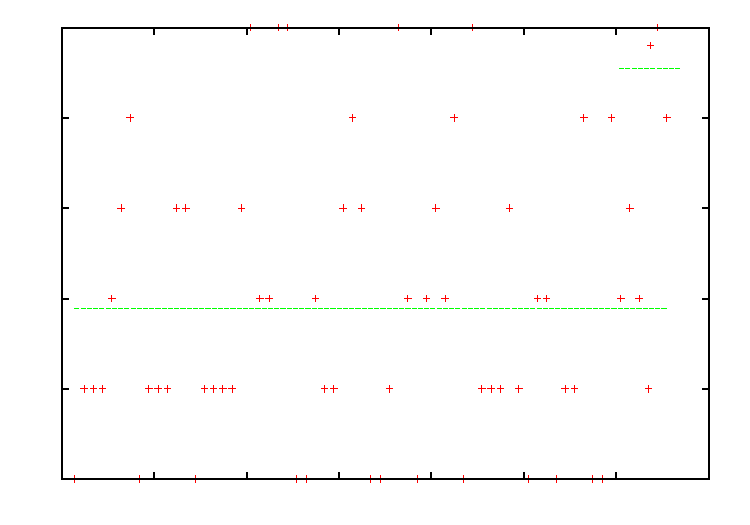
\includegraphics{null}}%
    \gplfronttext
  \end{picture}%
\endgroup

	\caption{Nullrate}
	\label{fig:null}
\end{figure}

\subsection{Halbwertszeit}
\begin{figure}[h]
\centering
% GNUPLOT: LaTeX picture with Postscript
\begingroup
  \makeatletter
  \providecommand\color[2][]{%
    \GenericError{(gnuplot) \space\space\space\@spaces}{%
      Package color not loaded in conjunction with
      terminal option `colourtext'%
    }{See the gnuplot documentation for explanation.%
    }{Either use 'blacktext' in gnuplot or load the package
      color.sty in LaTeX.}%
    \renewcommand\color[2][]{}%
  }%
  \providecommand\includegraphics[2][]{%
    \GenericError{(gnuplot) \space\space\space\@spaces}{%
      Package graphicx or graphics not loaded%
    }{See the gnuplot documentation for explanation.%
    }{The gnuplot epslatex terminal needs graphicx.sty or graphics.sty.}%
    \renewcommand\includegraphics[2][]{}%
  }%
  \providecommand\rotatebox[2]{#2}%
  \@ifundefined{ifGPcolor}{%
    \newif\ifGPcolor
    \GPcolortrue
  }{}%
  \@ifundefined{ifGPblacktext}{%
    \newif\ifGPblacktext
    \GPblacktexttrue
  }{}%
  % define a \g@addto@macro without @ in the name:
  \let\gplgaddtomacro\g@addto@macro
  % define empty templates for all commands taking text:
  \gdef\gplbacktext{}%
  \gdef\gplfronttext{}%
  \makeatother
  \ifGPblacktext
    % no textcolor at all
    \def\colorrgb#1{}%
    \def\colorgray#1{}%
  \else
    % gray or color?
    \ifGPcolor
      \def\colorrgb#1{\color[rgb]{#1}}%
      \def\colorgray#1{\color[gray]{#1}}%
      \expandafter\def\csname LTw\endcsname{\color{white}}%
      \expandafter\def\csname LTb\endcsname{\color{black}}%
      \expandafter\def\csname LTa\endcsname{\color{black}}%
      \expandafter\def\csname LT0\endcsname{\color[rgb]{1,0,0}}%
      \expandafter\def\csname LT1\endcsname{\color[rgb]{0,1,0}}%
      \expandafter\def\csname LT2\endcsname{\color[rgb]{0,0,1}}%
      \expandafter\def\csname LT3\endcsname{\color[rgb]{1,0,1}}%
      \expandafter\def\csname LT4\endcsname{\color[rgb]{0,1,1}}%
      \expandafter\def\csname LT5\endcsname{\color[rgb]{1,1,0}}%
      \expandafter\def\csname LT6\endcsname{\color[rgb]{0,0,0}}%
      \expandafter\def\csname LT7\endcsname{\color[rgb]{1,0.3,0}}%
      \expandafter\def\csname LT8\endcsname{\color[rgb]{0.5,0.5,0.5}}%
    \else
      % gray
      \def\colorrgb#1{\color{black}}%
      \def\colorgray#1{\color[gray]{#1}}%
      \expandafter\def\csname LTw\endcsname{\color{white}}%
      \expandafter\def\csname LTb\endcsname{\color{black}}%
      \expandafter\def\csname LTa\endcsname{\color{black}}%
      \expandafter\def\csname LT0\endcsname{\color{black}}%
      \expandafter\def\csname LT1\endcsname{\color{black}}%
      \expandafter\def\csname LT2\endcsname{\color{black}}%
      \expandafter\def\csname LT3\endcsname{\color{black}}%
      \expandafter\def\csname LT4\endcsname{\color{black}}%
      \expandafter\def\csname LT5\endcsname{\color{black}}%
      \expandafter\def\csname LT6\endcsname{\color{black}}%
      \expandafter\def\csname LT7\endcsname{\color{black}}%
      \expandafter\def\csname LT8\endcsname{\color{black}}%
    \fi
  \fi
  \setlength{\unitlength}{0.0500bp}%
  \begin{picture}(7200.00,5040.00)%
    \gplgaddtomacro\gplbacktext{%
      \csname LTb\endcsname%
      \put(946,934){\makebox(0,0)[r]{\strut{} 0}}%
      \put(946,1393){\makebox(0,0)[r]{\strut{} 20}}%
      \put(946,1852){\makebox(0,0)[r]{\strut{} 40}}%
      \put(946,2312){\makebox(0,0)[r]{\strut{} 60}}%
      \put(946,2771){\makebox(0,0)[r]{\strut{} 80}}%
      \put(946,3231){\makebox(0,0)[r]{\strut{} 100}}%
      \put(946,3690){\makebox(0,0)[r]{\strut{} 120}}%
      \put(946,4149){\makebox(0,0)[r]{\strut{} 140}}%
      \put(1078,484){\makebox(0,0){\strut{} 0}}%
      \put(2223,484){\makebox(0,0){\strut{} 50}}%
      \put(3368,484){\makebox(0,0){\strut{} 100}}%
      \put(4513,484){\makebox(0,0){\strut{} 150}}%
      \put(5658,484){\makebox(0,0){\strut{} 200}}%
      \put(6803,484){\makebox(0,0){\strut{} 250}}%
      \put(176,2541){\rotatebox{-270}{\makebox(0,0){\strut{}Anzahl der Zerfälle pro Sekunde $N$}}}%
      \put(3940,154){\makebox(0,0){\strut{}Zeit $t$ [s]}}%
      \put(3940,4709){\makebox(0,0){\strut{}Übersicht}}%
    }%
    \gplgaddtomacro\gplfronttext{%
      \csname LTb\endcsname%
      \put(5816,4206){\makebox(0,0)[r]{\strut{}fit 1 min}}%
      \csname LTb\endcsname%
      \put(5816,3986){\makebox(0,0)[r]{\strut{}fit 2 min}}%
      \csname LTb\endcsname%
      \put(5816,3766){\makebox(0,0)[r]{\strut{}fit 4 min}}%
      \csname LTb\endcsname%
      \put(5816,3546){\makebox(0,0)[r]{\strut{}fit 8 min}}%
      \csname LTb\endcsname%
      \put(5816,3326){\makebox(0,0)[r]{\strut{}fit Nullrate}}%
      \csname LTb\endcsname%
      \put(5816,3106){\makebox(0,0)[r]{\strut{}Messwerte 1min}}%
      \csname LTb\endcsname%
      \put(5816,2886){\makebox(0,0)[r]{\strut{}Messwerte 2min}}%
      \csname LTb\endcsname%
      \put(5816,2666){\makebox(0,0)[r]{\strut{}Messwerte 4 min}}%
      \csname LTb\endcsname%
      \put(5816,2446){\makebox(0,0)[r]{\strut{}Messwerte 8 min}}%
      \csname LTb\endcsname%
      \put(5816,2226){\makebox(0,0)[r]{\strut{}Messwerte Nullrate}}%
    }%
    \gplbacktext
    \put(0,0){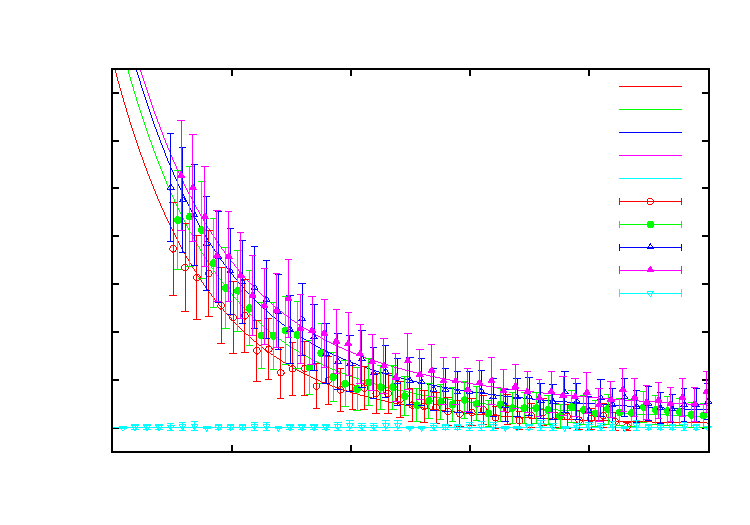
\includegraphics{plot1}}%
    \gplfronttext
  \end{picture}%
\endgroup

\caption{Alle Zerfallsreihen in einem Plot zusammengefasst}
\label{fig:alle}
\end{figure}
\begin{figure}[h]
\centering
% GNUPLOT: LaTeX picture with Postscript
\begingroup
  \makeatletter
  \providecommand\color[2][]{%
    \GenericError{(gnuplot) \space\space\space\@spaces}{%
      Package color not loaded in conjunction with
      terminal option `colourtext'%
    }{See the gnuplot documentation for explanation.%
    }{Either use 'blacktext' in gnuplot or load the package
      color.sty in LaTeX.}%
    \renewcommand\color[2][]{}%
  }%
  \providecommand\includegraphics[2][]{%
    \GenericError{(gnuplot) \space\space\space\@spaces}{%
      Package graphicx or graphics not loaded%
    }{See the gnuplot documentation for explanation.%
    }{The gnuplot epslatex terminal needs graphicx.sty or graphics.sty.}%
    \renewcommand\includegraphics[2][]{}%
  }%
  \providecommand\rotatebox[2]{#2}%
  \@ifundefined{ifGPcolor}{%
    \newif\ifGPcolor
    \GPcolortrue
  }{}%
  \@ifundefined{ifGPblacktext}{%
    \newif\ifGPblacktext
    \GPblacktexttrue
  }{}%
  % define a \g@addto@macro without @ in the name:
  \let\gplgaddtomacro\g@addto@macro
  % define empty templates for all commands taking text:
  \gdef\gplbacktext{}%
  \gdef\gplfronttext{}%
  \makeatother
  \ifGPblacktext
    % no textcolor at all
    \def\colorrgb#1{}%
    \def\colorgray#1{}%
  \else
    % gray or color?
    \ifGPcolor
      \def\colorrgb#1{\color[rgb]{#1}}%
      \def\colorgray#1{\color[gray]{#1}}%
      \expandafter\def\csname LTw\endcsname{\color{white}}%
      \expandafter\def\csname LTb\endcsname{\color{black}}%
      \expandafter\def\csname LTa\endcsname{\color{black}}%
      \expandafter\def\csname LT0\endcsname{\color[rgb]{1,0,0}}%
      \expandafter\def\csname LT1\endcsname{\color[rgb]{0,1,0}}%
      \expandafter\def\csname LT2\endcsname{\color[rgb]{0,0,1}}%
      \expandafter\def\csname LT3\endcsname{\color[rgb]{1,0,1}}%
      \expandafter\def\csname LT4\endcsname{\color[rgb]{0,1,1}}%
      \expandafter\def\csname LT5\endcsname{\color[rgb]{1,1,0}}%
      \expandafter\def\csname LT6\endcsname{\color[rgb]{0,0,0}}%
      \expandafter\def\csname LT7\endcsname{\color[rgb]{1,0.3,0}}%
      \expandafter\def\csname LT8\endcsname{\color[rgb]{0.5,0.5,0.5}}%
    \else
      % gray
      \def\colorrgb#1{\color{black}}%
      \def\colorgray#1{\color[gray]{#1}}%
      \expandafter\def\csname LTw\endcsname{\color{white}}%
      \expandafter\def\csname LTb\endcsname{\color{black}}%
      \expandafter\def\csname LTa\endcsname{\color{black}}%
      \expandafter\def\csname LT0\endcsname{\color{black}}%
      \expandafter\def\csname LT1\endcsname{\color{black}}%
      \expandafter\def\csname LT2\endcsname{\color{black}}%
      \expandafter\def\csname LT3\endcsname{\color{black}}%
      \expandafter\def\csname LT4\endcsname{\color{black}}%
      \expandafter\def\csname LT5\endcsname{\color{black}}%
      \expandafter\def\csname LT6\endcsname{\color{black}}%
      \expandafter\def\csname LT7\endcsname{\color{black}}%
      \expandafter\def\csname LT8\endcsname{\color{black}}%
    \fi
  \fi
  \setlength{\unitlength}{0.0500bp}%
  \begin{picture}(7200.00,5040.00)%
    \gplgaddtomacro\gplbacktext{%
      \csname LTb\endcsname%
      \put(946,934){\makebox(0,0)[r]{\strut{} 0}}%
      \put(946,1393){\makebox(0,0)[r]{\strut{} 20}}%
      \put(946,1852){\makebox(0,0)[r]{\strut{} 40}}%
      \put(946,2312){\makebox(0,0)[r]{\strut{} 60}}%
      \put(946,2771){\makebox(0,0)[r]{\strut{} 80}}%
      \put(946,3231){\makebox(0,0)[r]{\strut{} 100}}%
      \put(946,3690){\makebox(0,0)[r]{\strut{} 120}}%
      \put(946,4149){\makebox(0,0)[r]{\strut{} 140}}%
      \put(1078,484){\makebox(0,0){\strut{} 0}}%
      \put(2223,484){\makebox(0,0){\strut{} 50}}%
      \put(3368,484){\makebox(0,0){\strut{} 100}}%
      \put(4513,484){\makebox(0,0){\strut{} 150}}%
      \put(5658,484){\makebox(0,0){\strut{} 200}}%
      \put(6803,484){\makebox(0,0){\strut{} 250}}%
      \put(176,2541){\rotatebox{-270}{\makebox(0,0){\strut{}Anzahl der Zerfälle pro Sekunde $N$}}}%
      \put(3940,154){\makebox(0,0){\strut{}Zeit $t$ [s]}}%
      \put(3940,4709){\makebox(0,0){\strut{}1 Minute Aktivierungszeit}}%
    }%
    \gplgaddtomacro\gplfronttext{%
      \csname LTb\endcsname%
      \put(5816,4206){\makebox(0,0)[r]{\strut{}Isotop A}}%
      \csname LTb\endcsname%
      \put(5816,3986){\makebox(0,0)[r]{\strut{}Isotop B}}%
      \csname LTb\endcsname%
      \put(5816,3766){\makebox(0,0)[r]{\strut{}Summe}}%
      \csname LTb\endcsname%
      \put(5816,3546){\makebox(0,0)[r]{\strut{}Nullrate}}%
      \csname LTb\endcsname%
      \put(5816,3326){\makebox(0,0)[r]{\strut{}Messwerte 1 min}}%
    }%
    \gplbacktext
    \put(0,0){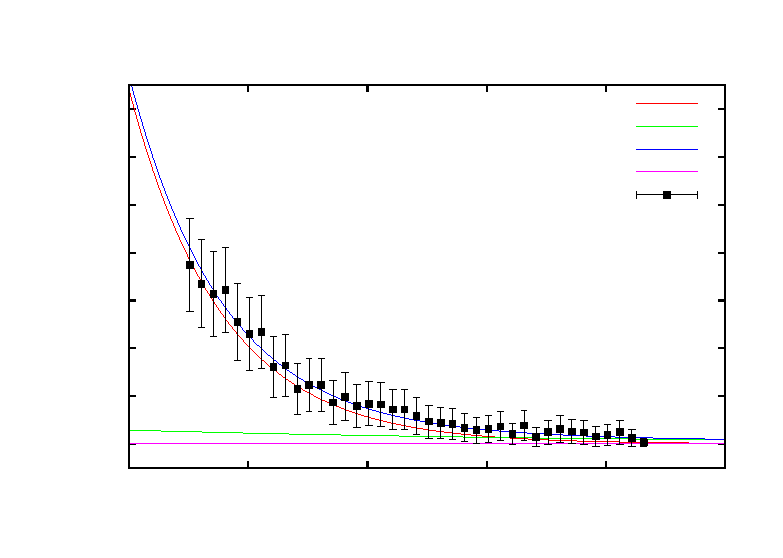
\includegraphics{plot1min}}%
    \gplfronttext
  \end{picture}%
\endgroup

\caption{Zerfallsrate für ein Minute Aktivierung}
\label{fig:1min}
\end{figure}

\begin{figure}[h]
\centering
% GNUPLOT: LaTeX picture with Postscript
\begingroup
  \makeatletter
  \providecommand\color[2][]{%
    \GenericError{(gnuplot) \space\space\space\@spaces}{%
      Package color not loaded in conjunction with
      terminal option `colourtext'%
    }{See the gnuplot documentation for explanation.%
    }{Either use 'blacktext' in gnuplot or load the package
      color.sty in LaTeX.}%
    \renewcommand\color[2][]{}%
  }%
  \providecommand\includegraphics[2][]{%
    \GenericError{(gnuplot) \space\space\space\@spaces}{%
      Package graphicx or graphics not loaded%
    }{See the gnuplot documentation for explanation.%
    }{The gnuplot epslatex terminal needs graphicx.sty or graphics.sty.}%
    \renewcommand\includegraphics[2][]{}%
  }%
  \providecommand\rotatebox[2]{#2}%
  \@ifundefined{ifGPcolor}{%
    \newif\ifGPcolor
    \GPcolortrue
  }{}%
  \@ifundefined{ifGPblacktext}{%
    \newif\ifGPblacktext
    \GPblacktexttrue
  }{}%
  % define a \g@addto@macro without @ in the name:
  \let\gplgaddtomacro\g@addto@macro
  % define empty templates for all commands taking text:
  \gdef\gplbacktext{}%
  \gdef\gplfronttext{}%
  \makeatother
  \ifGPblacktext
    % no textcolor at all
    \def\colorrgb#1{}%
    \def\colorgray#1{}%
  \else
    % gray or color?
    \ifGPcolor
      \def\colorrgb#1{\color[rgb]{#1}}%
      \def\colorgray#1{\color[gray]{#1}}%
      \expandafter\def\csname LTw\endcsname{\color{white}}%
      \expandafter\def\csname LTb\endcsname{\color{black}}%
      \expandafter\def\csname LTa\endcsname{\color{black}}%
      \expandafter\def\csname LT0\endcsname{\color[rgb]{1,0,0}}%
      \expandafter\def\csname LT1\endcsname{\color[rgb]{0,1,0}}%
      \expandafter\def\csname LT2\endcsname{\color[rgb]{0,0,1}}%
      \expandafter\def\csname LT3\endcsname{\color[rgb]{1,0,1}}%
      \expandafter\def\csname LT4\endcsname{\color[rgb]{0,1,1}}%
      \expandafter\def\csname LT5\endcsname{\color[rgb]{1,1,0}}%
      \expandafter\def\csname LT6\endcsname{\color[rgb]{0,0,0}}%
      \expandafter\def\csname LT7\endcsname{\color[rgb]{1,0.3,0}}%
      \expandafter\def\csname LT8\endcsname{\color[rgb]{0.5,0.5,0.5}}%
    \else
      % gray
      \def\colorrgb#1{\color{black}}%
      \def\colorgray#1{\color[gray]{#1}}%
      \expandafter\def\csname LTw\endcsname{\color{white}}%
      \expandafter\def\csname LTb\endcsname{\color{black}}%
      \expandafter\def\csname LTa\endcsname{\color{black}}%
      \expandafter\def\csname LT0\endcsname{\color{black}}%
      \expandafter\def\csname LT1\endcsname{\color{black}}%
      \expandafter\def\csname LT2\endcsname{\color{black}}%
      \expandafter\def\csname LT3\endcsname{\color{black}}%
      \expandafter\def\csname LT4\endcsname{\color{black}}%
      \expandafter\def\csname LT5\endcsname{\color{black}}%
      \expandafter\def\csname LT6\endcsname{\color{black}}%
      \expandafter\def\csname LT7\endcsname{\color{black}}%
      \expandafter\def\csname LT8\endcsname{\color{black}}%
    \fi
  \fi
  \setlength{\unitlength}{0.0500bp}%
  \begin{picture}(7200.00,5040.00)%
    \gplgaddtomacro\gplbacktext{%
      \csname LTb\endcsname%
      \put(946,934){\makebox(0,0)[r]{\strut{} 0}}%
      \put(946,1393){\makebox(0,0)[r]{\strut{} 20}}%
      \put(946,1852){\makebox(0,0)[r]{\strut{} 40}}%
      \put(946,2312){\makebox(0,0)[r]{\strut{} 60}}%
      \put(946,2771){\makebox(0,0)[r]{\strut{} 80}}%
      \put(946,3231){\makebox(0,0)[r]{\strut{} 100}}%
      \put(946,3690){\makebox(0,0)[r]{\strut{} 120}}%
      \put(946,4149){\makebox(0,0)[r]{\strut{} 140}}%
      \put(1078,484){\makebox(0,0){\strut{} 0}}%
      \put(2223,484){\makebox(0,0){\strut{} 50}}%
      \put(3368,484){\makebox(0,0){\strut{} 100}}%
      \put(4513,484){\makebox(0,0){\strut{} 150}}%
      \put(5658,484){\makebox(0,0){\strut{} 200}}%
      \put(6803,484){\makebox(0,0){\strut{} 250}}%
      \put(176,2541){\rotatebox{-270}{\makebox(0,0){\strut{}Anzahl der Zerfälle pro Sekunde $N$}}}%
      \put(3940,154){\makebox(0,0){\strut{}Zeit $t$ [s]}}%
      \put(3940,4709){\makebox(0,0){\strut{}2 Minuten Aktivierungszeit}}%
    }%
    \gplgaddtomacro\gplfronttext{%
      \csname LTb\endcsname%
      \put(5816,4206){\makebox(0,0)[r]{\strut{}Isotop A}}%
      \csname LTb\endcsname%
      \put(5816,3986){\makebox(0,0)[r]{\strut{}Isotop B}}%
      \csname LTb\endcsname%
      \put(5816,3766){\makebox(0,0)[r]{\strut{}Summe}}%
      \csname LTb\endcsname%
      \put(5816,3546){\makebox(0,0)[r]{\strut{}Nullrate}}%
      \csname LTb\endcsname%
      \put(5816,3326){\makebox(0,0)[r]{\strut{}Messwerte 2 min}}%
    }%
    \gplbacktext
    \put(0,0){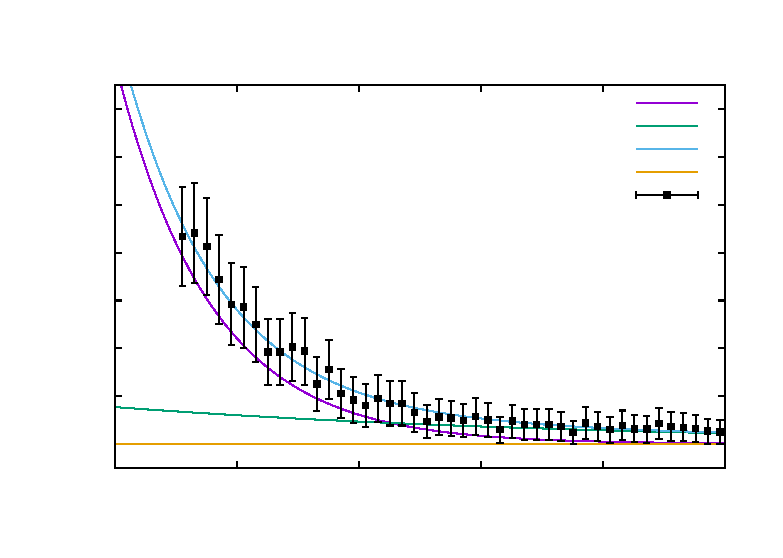
\includegraphics{plot2min}}%
    \gplfronttext
  \end{picture}%
\endgroup

\caption{Zerfallsrate für 2 Minuten Aktivierung}
\label{fig:2min}
\end{figure}

\begin{figure}[h]
\centering
% GNUPLOT: LaTeX picture with Postscript
\begingroup
  \makeatletter
  \providecommand\color[2][]{%
    \GenericError{(gnuplot) \space\space\space\@spaces}{%
      Package color not loaded in conjunction with
      terminal option `colourtext'%
    }{See the gnuplot documentation for explanation.%
    }{Either use 'blacktext' in gnuplot or load the package
      color.sty in LaTeX.}%
    \renewcommand\color[2][]{}%
  }%
  \providecommand\includegraphics[2][]{%
    \GenericError{(gnuplot) \space\space\space\@spaces}{%
      Package graphicx or graphics not loaded%
    }{See the gnuplot documentation for explanation.%
    }{The gnuplot epslatex terminal needs graphicx.sty or graphics.sty.}%
    \renewcommand\includegraphics[2][]{}%
  }%
  \providecommand\rotatebox[2]{#2}%
  \@ifundefined{ifGPcolor}{%
    \newif\ifGPcolor
    \GPcolortrue
  }{}%
  \@ifundefined{ifGPblacktext}{%
    \newif\ifGPblacktext
    \GPblacktexttrue
  }{}%
  % define a \g@addto@macro without @ in the name:
  \let\gplgaddtomacro\g@addto@macro
  % define empty templates for all commands taking text:
  \gdef\gplbacktext{}%
  \gdef\gplfronttext{}%
  \makeatother
  \ifGPblacktext
    % no textcolor at all
    \def\colorrgb#1{}%
    \def\colorgray#1{}%
  \else
    % gray or color?
    \ifGPcolor
      \def\colorrgb#1{\color[rgb]{#1}}%
      \def\colorgray#1{\color[gray]{#1}}%
      \expandafter\def\csname LTw\endcsname{\color{white}}%
      \expandafter\def\csname LTb\endcsname{\color{black}}%
      \expandafter\def\csname LTa\endcsname{\color{black}}%
      \expandafter\def\csname LT0\endcsname{\color[rgb]{1,0,0}}%
      \expandafter\def\csname LT1\endcsname{\color[rgb]{0,1,0}}%
      \expandafter\def\csname LT2\endcsname{\color[rgb]{0,0,1}}%
      \expandafter\def\csname LT3\endcsname{\color[rgb]{1,0,1}}%
      \expandafter\def\csname LT4\endcsname{\color[rgb]{0,1,1}}%
      \expandafter\def\csname LT5\endcsname{\color[rgb]{1,1,0}}%
      \expandafter\def\csname LT6\endcsname{\color[rgb]{0,0,0}}%
      \expandafter\def\csname LT7\endcsname{\color[rgb]{1,0.3,0}}%
      \expandafter\def\csname LT8\endcsname{\color[rgb]{0.5,0.5,0.5}}%
    \else
      % gray
      \def\colorrgb#1{\color{black}}%
      \def\colorgray#1{\color[gray]{#1}}%
      \expandafter\def\csname LTw\endcsname{\color{white}}%
      \expandafter\def\csname LTb\endcsname{\color{black}}%
      \expandafter\def\csname LTa\endcsname{\color{black}}%
      \expandafter\def\csname LT0\endcsname{\color{black}}%
      \expandafter\def\csname LT1\endcsname{\color{black}}%
      \expandafter\def\csname LT2\endcsname{\color{black}}%
      \expandafter\def\csname LT3\endcsname{\color{black}}%
      \expandafter\def\csname LT4\endcsname{\color{black}}%
      \expandafter\def\csname LT5\endcsname{\color{black}}%
      \expandafter\def\csname LT6\endcsname{\color{black}}%
      \expandafter\def\csname LT7\endcsname{\color{black}}%
      \expandafter\def\csname LT8\endcsname{\color{black}}%
    \fi
  \fi
  \setlength{\unitlength}{0.0500bp}%
  \begin{picture}(7200.00,5040.00)%
    \gplgaddtomacro\gplbacktext{%
      \csname LTb\endcsname%
      \put(946,934){\makebox(0,0)[r]{\strut{} 0}}%
      \put(946,1393){\makebox(0,0)[r]{\strut{} 20}}%
      \put(946,1852){\makebox(0,0)[r]{\strut{} 40}}%
      \put(946,2312){\makebox(0,0)[r]{\strut{} 60}}%
      \put(946,2771){\makebox(0,0)[r]{\strut{} 80}}%
      \put(946,3231){\makebox(0,0)[r]{\strut{} 100}}%
      \put(946,3690){\makebox(0,0)[r]{\strut{} 120}}%
      \put(946,4149){\makebox(0,0)[r]{\strut{} 140}}%
      \put(1078,484){\makebox(0,0){\strut{} 0}}%
      \put(2223,484){\makebox(0,0){\strut{} 50}}%
      \put(3368,484){\makebox(0,0){\strut{} 100}}%
      \put(4513,484){\makebox(0,0){\strut{} 150}}%
      \put(5658,484){\makebox(0,0){\strut{} 200}}%
      \put(6803,484){\makebox(0,0){\strut{} 250}}%
      \put(176,2541){\rotatebox{-270}{\makebox(0,0){\strut{}Anzahl der Zerfälle pro Sekunde $N$}}}%
      \put(3940,154){\makebox(0,0){\strut{}Zeit $t$ [s]}}%
      \put(3940,4709){\makebox(0,0){\strut{}4 Minuten Aktivierungszeit}}%
    }%
    \gplgaddtomacro\gplfronttext{%
      \csname LTb\endcsname%
      \put(5816,4206){\makebox(0,0)[r]{\strut{}Isotop A}}%
      \csname LTb\endcsname%
      \put(5816,3986){\makebox(0,0)[r]{\strut{}Isotop B}}%
      \csname LTb\endcsname%
      \put(5816,3766){\makebox(0,0)[r]{\strut{}Summe}}%
      \csname LTb\endcsname%
      \put(5816,3546){\makebox(0,0)[r]{\strut{}Nullrate}}%
      \csname LTb\endcsname%
      \put(5816,3326){\makebox(0,0)[r]{\strut{}Messwerte 4 min}}%
    }%
    \gplbacktext
    \put(0,0){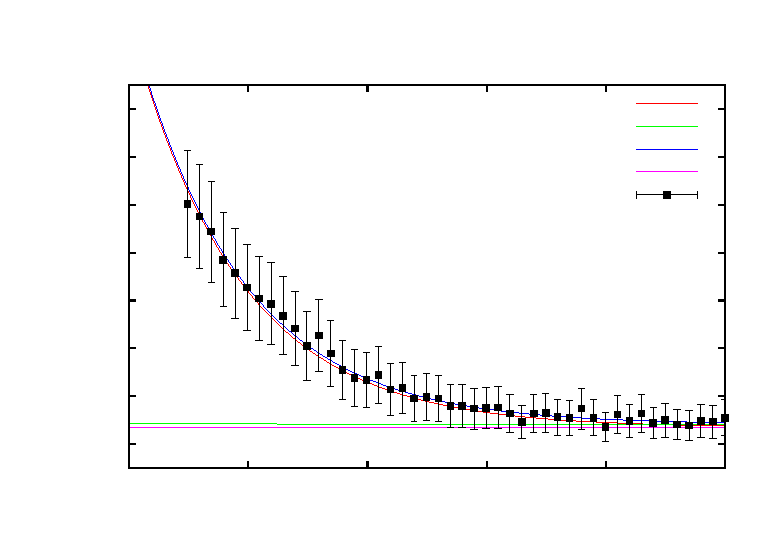
\includegraphics{plot4min}}%
    \gplfronttext
  \end{picture}%
\endgroup

\caption{Zerfallsrate für 4 Minuten Aktivierung}
\label{fig:4min}
\end{figure}


\begin{figure}[h]
\centering
% GNUPLOT: LaTeX picture with Postscript
\begingroup
  \makeatletter
  \providecommand\color[2][]{%
    \GenericError{(gnuplot) \space\space\space\@spaces}{%
      Package color not loaded in conjunction with
      terminal option `colourtext'%
    }{See the gnuplot documentation for explanation.%
    }{Either use 'blacktext' in gnuplot or load the package
      color.sty in LaTeX.}%
    \renewcommand\color[2][]{}%
  }%
  \providecommand\includegraphics[2][]{%
    \GenericError{(gnuplot) \space\space\space\@spaces}{%
      Package graphicx or graphics not loaded%
    }{See the gnuplot documentation for explanation.%
    }{The gnuplot epslatex terminal needs graphicx.sty or graphics.sty.}%
    \renewcommand\includegraphics[2][]{}%
  }%
  \providecommand\rotatebox[2]{#2}%
  \@ifundefined{ifGPcolor}{%
    \newif\ifGPcolor
    \GPcolortrue
  }{}%
  \@ifundefined{ifGPblacktext}{%
    \newif\ifGPblacktext
    \GPblacktexttrue
  }{}%
  % define a \g@addto@macro without @ in the name:
  \let\gplgaddtomacro\g@addto@macro
  % define empty templates for all commands taking text:
  \gdef\gplbacktext{}%
  \gdef\gplfronttext{}%
  \makeatother
  \ifGPblacktext
    % no textcolor at all
    \def\colorrgb#1{}%
    \def\colorgray#1{}%
  \else
    % gray or color?
    \ifGPcolor
      \def\colorrgb#1{\color[rgb]{#1}}%
      \def\colorgray#1{\color[gray]{#1}}%
      \expandafter\def\csname LTw\endcsname{\color{white}}%
      \expandafter\def\csname LTb\endcsname{\color{black}}%
      \expandafter\def\csname LTa\endcsname{\color{black}}%
      \expandafter\def\csname LT0\endcsname{\color[rgb]{1,0,0}}%
      \expandafter\def\csname LT1\endcsname{\color[rgb]{0,1,0}}%
      \expandafter\def\csname LT2\endcsname{\color[rgb]{0,0,1}}%
      \expandafter\def\csname LT3\endcsname{\color[rgb]{1,0,1}}%
      \expandafter\def\csname LT4\endcsname{\color[rgb]{0,1,1}}%
      \expandafter\def\csname LT5\endcsname{\color[rgb]{1,1,0}}%
      \expandafter\def\csname LT6\endcsname{\color[rgb]{0,0,0}}%
      \expandafter\def\csname LT7\endcsname{\color[rgb]{1,0.3,0}}%
      \expandafter\def\csname LT8\endcsname{\color[rgb]{0.5,0.5,0.5}}%
    \else
      % gray
      \def\colorrgb#1{\color{black}}%
      \def\colorgray#1{\color[gray]{#1}}%
      \expandafter\def\csname LTw\endcsname{\color{white}}%
      \expandafter\def\csname LTb\endcsname{\color{black}}%
      \expandafter\def\csname LTa\endcsname{\color{black}}%
      \expandafter\def\csname LT0\endcsname{\color{black}}%
      \expandafter\def\csname LT1\endcsname{\color{black}}%
      \expandafter\def\csname LT2\endcsname{\color{black}}%
      \expandafter\def\csname LT3\endcsname{\color{black}}%
      \expandafter\def\csname LT4\endcsname{\color{black}}%
      \expandafter\def\csname LT5\endcsname{\color{black}}%
      \expandafter\def\csname LT6\endcsname{\color{black}}%
      \expandafter\def\csname LT7\endcsname{\color{black}}%
      \expandafter\def\csname LT8\endcsname{\color{black}}%
    \fi
  \fi
    \setlength{\unitlength}{0.0500bp}%
    \ifx\gptboxheight\undefined%
      \newlength{\gptboxheight}%
      \newlength{\gptboxwidth}%
      \newsavebox{\gptboxtext}%
    \fi%
    \setlength{\fboxrule}{0.5pt}%
    \setlength{\fboxsep}{1pt}%
\begin{picture}(7200.00,5040.00)%
    \gplgaddtomacro\gplbacktext{%
      \csname LTb\endcsname%
      \put(814,934){\makebox(0,0)[r]{\strut{}$0$}}%
      \put(814,1393){\makebox(0,0)[r]{\strut{}$20$}}%
      \put(814,1852){\makebox(0,0)[r]{\strut{}$40$}}%
      \put(814,2312){\makebox(0,0)[r]{\strut{}$60$}}%
      \put(814,2771){\makebox(0,0)[r]{\strut{}$80$}}%
      \put(814,3231){\makebox(0,0)[r]{\strut{}$100$}}%
      \put(814,3690){\makebox(0,0)[r]{\strut{}$120$}}%
      \put(814,4149){\makebox(0,0)[r]{\strut{}$140$}}%
      \put(946,484){\makebox(0,0){\strut{}$0$}}%
      \put(2117,484){\makebox(0,0){\strut{}$50$}}%
      \put(3289,484){\makebox(0,0){\strut{}$100$}}%
      \put(4460,484){\makebox(0,0){\strut{}$150$}}%
      \put(5632,484){\makebox(0,0){\strut{}$200$}}%
      \put(6803,484){\makebox(0,0){\strut{}$250$}}%
    }%
    \gplgaddtomacro\gplfronttext{%
      \csname LTb\endcsname%
      \put(176,2541){\rotatebox{-270}{\makebox(0,0){\strut{}Anzahl der Zerfälle pro Sekunde $N$}}}%
      \put(3874,154){\makebox(0,0){\strut{}Zeit $t$ [s]}}%
      \put(3874,4709){\makebox(0,0){\strut{}8 Minuten Aktivierungszeit}}%
      \csname LTb\endcsname%
      \put(5816,4206){\makebox(0,0)[r]{\strut{}Isotop A}}%
      \csname LTb\endcsname%
      \put(5816,3986){\makebox(0,0)[r]{\strut{}Isotop B}}%
      \csname LTb\endcsname%
      \put(5816,3766){\makebox(0,0)[r]{\strut{}Summe}}%
      \csname LTb\endcsname%
      \put(5816,3546){\makebox(0,0)[r]{\strut{}Nullrate}}%
      \csname LTb\endcsname%
      \put(5816,3326){\makebox(0,0)[r]{\strut{}Messwerte 8 min}}%
    }%
    \gplbacktext
    \put(0,0){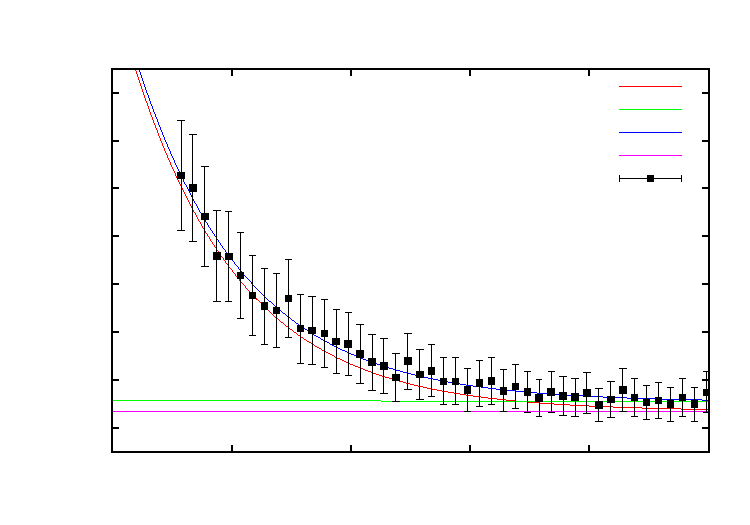
\includegraphics{plot8min}}%
    \gplfronttext
  \end{picture}%
\endgroup

\caption{Zerfallsrate für 8 Minuten Aktivierung}
\label{fig:8min}
\end{figure}





\section{Diskussion}
\label{sec:diskussion}

\bibliography{literatur}
\bibliographystyle{babalpha}
\end{document}
